\section{Kompetenzen von Skills} \label{Skillkompetenzen}
	Für die Definition eines Skills wird nicht die Funktion des Gesamtsystem so weit wie möglich in Teilfunktionalitäten heruntergebrochen, sondern die Funktionalitäten der Komponenten im System. Dabei betrachtet man jeden Komponenten-Typ, so weit wie möglich, einzeln (\ref{fig:Skillintegration}). Der Vorteil dieser Definition ist, dass für neue oder angepasste Systeme dieselben Skills eingesetzt werden können. Ein Robotersystem hat in jeder Anlage die identischen Grundfunktionalitäten und somit Skills. Der Skill ist anwendungsunabhängig. Die aus den Skills erstellten Sequenzen bilden die Funktion der Anwendung ab. Damit unterscheidet sich die Definierung der Skills von vergleichbaren Projekten wie z.B. der bereits durchgeführten Master-Thesis auf Basis von ROS (Ref). Dort haben Skills Funktionalitäten von mehreren Komponenten ineinander kombiniert, wodurch der Skill stärker an das spezifische System gebunden war.
	\begin{figure}[h!]
		\centering
		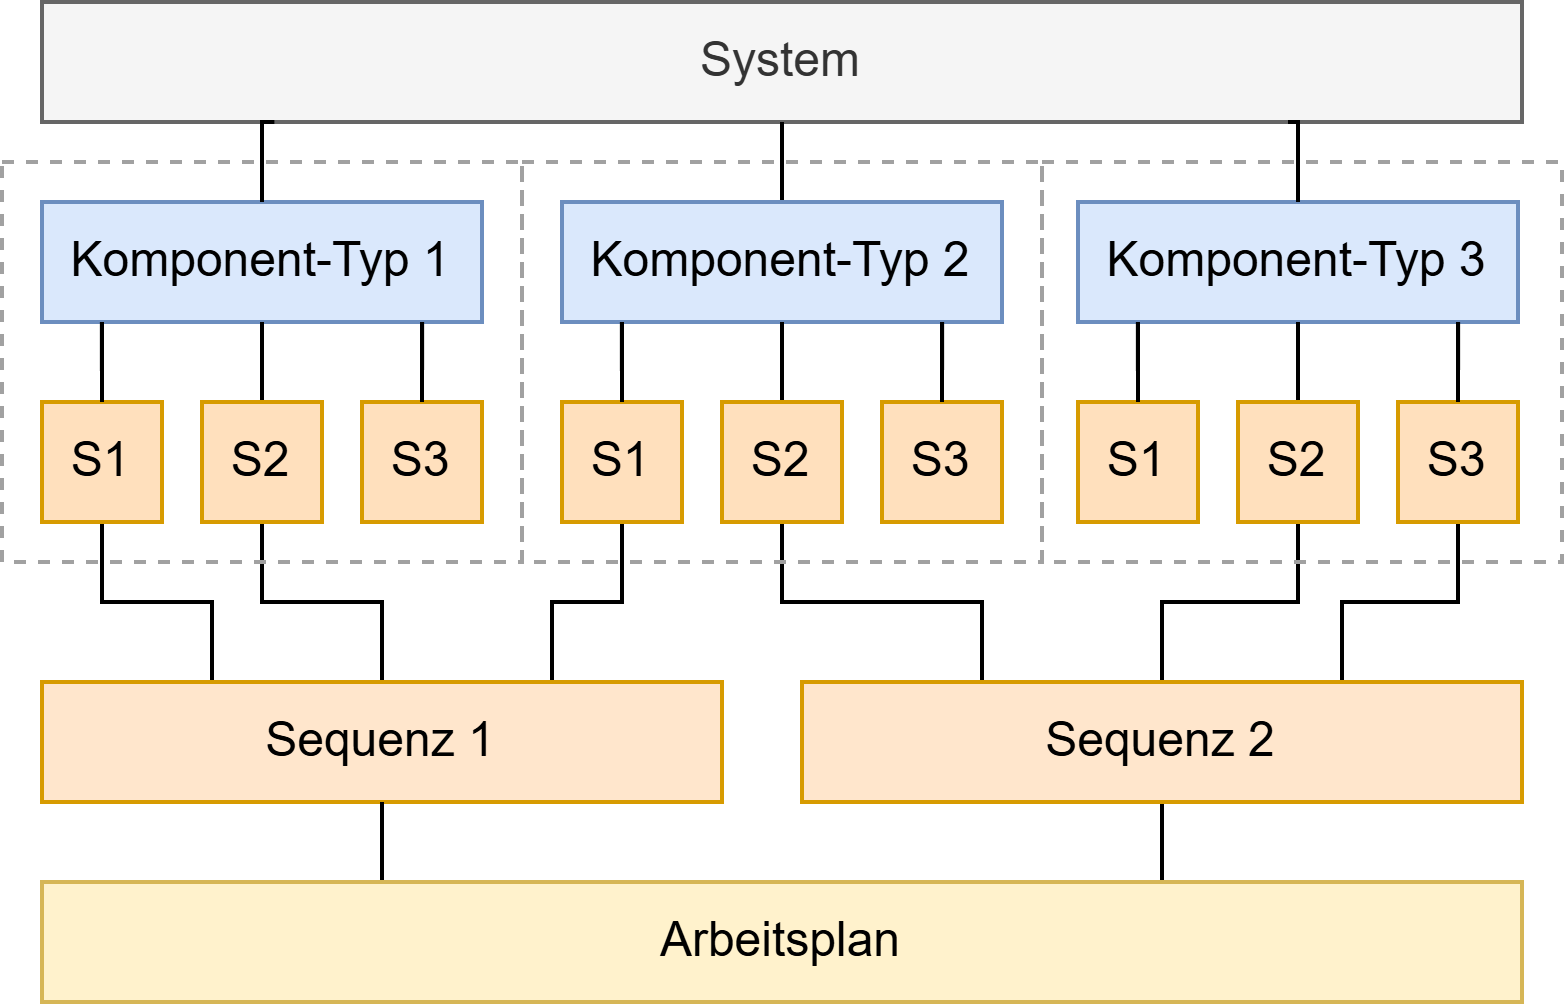
\includegraphics[width=0.7\textwidth]{06_Skillentwicklung/Skillkompetenzen}
		\captionsetup{justification=centering}
		\caption{Skill-Integration in System}
		\label{fig:Skillintegration}
	\end{figure}
	
	Die Kompetenzen eines Skills lassen sich in vier Bereiche aufteilen: 
	
	\begin{tabularx}{\textwidth}{@{}>{}p{8em} X@{}}
		Zuweisung: & 
		Der Skills ist für die Zuweisung einer Komponente zuständig. Es muss definiert werden können, welche Komponente den Skill ausführt.
		\\
		Umsetzung: & 
		Die definierte Grundfunktion muss innerhalb des Skills umgesetzt werden. Der Skill muss mittels Parameter-Inputs flexibel eingesetzt werden können.
		\\
		Verarbeitung: & 
		Die Informationen der Grundfunktion wird so ausgegeben, dass das Anlagenobjekt damit arbeiten und die reale Komponente ansteuern kann.
		\\
		Auswertung: & 
		Die momentane Situation der Komponente wird überwacht und ausgewertet. Der Skill kann auf bestimmte Situationen reagieren. 
		\\
	\end{tabularx}